
\documentclass[9pt,a4paper]{article}
\usepackage[left=1cm,right=1cm,top=1.2cm,bottom=1.2cm]{geometry}
\usepackage[utf8]{inputenc}
\usepackage{multicol}
\usepackage{fancyhdr}
\usepackage{listings}
\usepackage{xcolor}
\usepackage{titlesec}
\usepackage{graphicx}
\graphicspath{{./pics/}}
\usepackage{parskip}
\usepackage{caption}
\usepackage{enumitem}
\usepackage{tikz}
% \usepackage[hidelinks]{hyperref}
\usepackage[]{hyperref}
% \usepackage[utf8]{inputenc}
\usepackage[T1]{fontenc}
\usepackage[ngerman]{babel}
% \usepackage{minted}
\usepackage{float}
\usepackage{amsmath}
\usepackage{wrapfig}
\usepackage{pgfplots}
\usepackage{booktabs}
\usepackage{amssymb}
\usepackage{cancel}
\usepackage{pdfpages}

\usetikzlibrary{positioning}

% Querformat und kompaktes Layout
\pagestyle{fancy}
\fancyhf{}
\fancyfoot[RO]{\thepage}

\setlist[itemize]{nosep,left=0.1cm}  %- kompakte und eingerueckte Listen
\setlist[enumerate]{nosep,left=0.1cm} % aehnlich fuer nummerierte Listen, falls benoetigt

% Abstaende fuer Sektionen nach VHDL-Vorlage [2]
\titlespacing*{\section}{0pt}{0.3em}{0.2em}
\titlespacing*{\subsection}{0pt}{0.2em}{0.1em}
\setlength{\columnsep}{1cm} % - Abstand zwischen Spalten
\setlength{\columnseprule}{0.4pt} % - Linie zwischen Spalten

% Titelformatierung fuer Subsektionen
\titleformat{\subsection}{\bfseries\small}{\thesubsection}{1em}{}

% Farben fuer C++-Syntax-Highlighting
\definecolor{cppkeyword}{rgb}{0.1,0.1,0.7} % Blau-Violett
\definecolor{cpptype}{rgb}{0.4,0.1,0.6} % Violett
\definecolor{cppconcept}{rgb}{0.0,0.5,0.3} % Gruen
\definecolor{cppcomment}{rgb}{0.5,0.5,0.5} % Grau
\definecolor{cppstring}{rgb}{0.7,0.4,0.1} % Orange
\definecolor{cppbackground}{rgb}{0.98, 0.98, 0.98} % Grau
\definecolor{cppframe}{rgb}{0.8,0.8,0.8} % Grau

% Listing-Stil fuer C++
\lstdefinestyle{cppstyle}{
	language=C++, % Sprache C++
	basicstyle=\ttfamily\scriptsize, % - Schriftart und Groesse
	keywordstyle=\color{cppkeyword}\bfseries, % - Schluesselwoerter fett und farbig
	commentstyle=\color{cppcomment}\itshape, % - Kommentare kursiv und farbig
	stringstyle=\color{cppstring}, % - Strings farbig
	backgroundcolor=\color{cppbackground}, % - Hintergrundfarbe
	frame=lines, % - Rahmen
	rulecolor=\color{cppframe}, % - Rahmenfarbe
	breaklines=true, % - Zeilenumbrueche erlauben
	tabsize=2, % - Tabulatorgroesse
	columns=fullflexible, % - Spaltenmodus
	% Weitere Schluesselwoerter und hervorgehobene Typen fuer C++
	morekeywords={ % [4]
			alignas, alignof, and, and_eq, asm, auto, bitand, bitor,
			bool, break, case, catch, char, char16_t, char32_t, class,
			compl, concept, const, constexpr, const_cast, continue,
			decltype, default, delete, do, double, dynamic_cast, else,
			enum, explicit, export, extern, false, float, for, friend,
			goto, if, inline, int, long, mutable, namespace, new, noexcept,
			not, not_eq, nullptr, operator, or, or_eq, private, protected,
			public, register, reinterpret_cast, requires, return, short,
			signed, sizeof, static, static_assert, static_cast, struct,
			switch, template, this, thread_local, throw, true, try,
			typedef, typeid, typename, union, unsigned, using, virtual,
			void, volatile, wchar_t, while, xor, xor_eq, final, override
		},
	emph={ % - Hervorgehobene Typen/Konzepte
			int, double, char, bool, void, std::string, std::vector,
			std::list, std::map, std::set, std::iostream, std::fstream,
			std::strstream, std::iomanip, std::endl, std::cout, std::cin, std::cerr,
			std::exception, std::invalid_argument, std::runtime_error
		},
	emphstyle=\color{cpptype}, % - Stil fuer hervorgehobene Typen
	emph={[2]std::begin, std::end, std::sort, std::for_each,
			malloc, free, new, delete, connect, QObject, QWidget, QPainter,
			typeid, dynamic_cast, static_cast, reinterpret_cast, const_cast}, % - Hervorgehobene Funktionen/Konzeptebene 2
	emphstyle={[2]\color{cppconcept}\bfseries} % - Stil fuer Hervorgehobene Funktionen/Konzeptebene 2
}

\lstset{style=cppstyle}
\newcommand{\sourcecite}[1]{{\small\textsuperscript{[#1]}}} % Fuegt die Zitate als hochgestellte Zahl in Klammern ein

% install libaries with: sudo dnf install texlive-scheme-medium
% compile with: pdflatex -shell-escape dsp_cheatsheet.tex

\begin{document}
\begin{center}{\vspace{-4cm}
		\LARGE \textbf{VHF Tranceiver for CUBSAT Applications}}\\
	\small Fynn Gewiese | \href{https://github.com/Flynsky}{github}\\
	\rule{\linewidth}{0.3pt}
\end{center}

% \begin{multicols*}{2}
\raggedcolumns{\small\tableofcontents}

\section{Overview}

\subsection{Requirements}
\begin{minipage}{0.45\textwidth}
	\begin{itemize}
		\item Frequency Band: 134--174\,MHz (VHF)
		\item Data Rate: > 1k bps
		\item Tx Power: 0.3\,W / -5.2 dBW / 25.8 dBm
		\item Antenna Gain Satellite: >= 2.2 dBi
		\item Sattellite Effective Isotropic Radiated Power: -5.3 dBW
		\item Rx Sensitivity:
		\item TCXO Temperature Compensated Crystal Oscillator
	\end{itemize}
\end{minipage}
\hfill
\begin{minipage}{0.5\textwidth}
	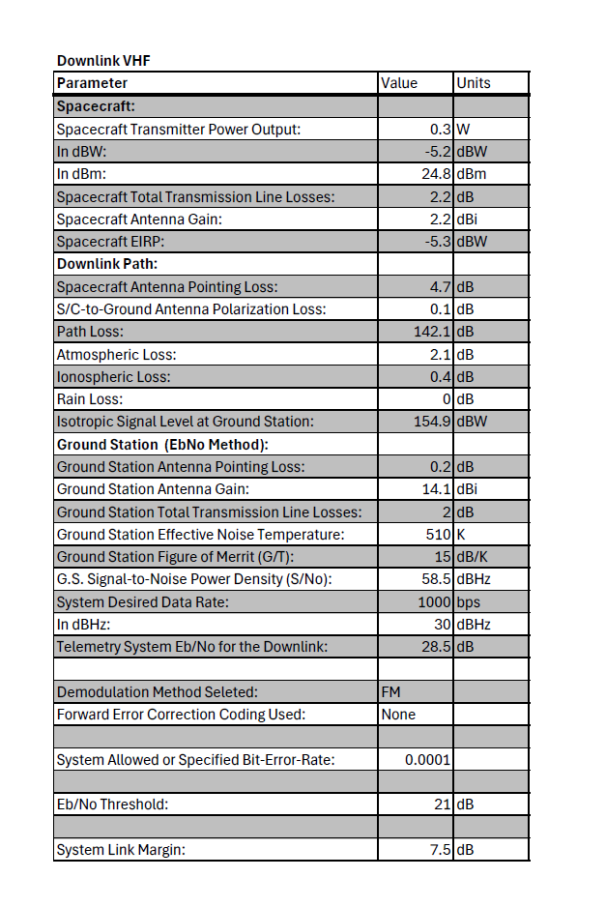
\includegraphics[width=\linewidth]{assets/RequireGroundstation.png}
	{Random Requirements from Christian}
\end{minipage}

\section{Transceiver}


Friis Power Estimate:
\begin{figure}[h]
	\centering
	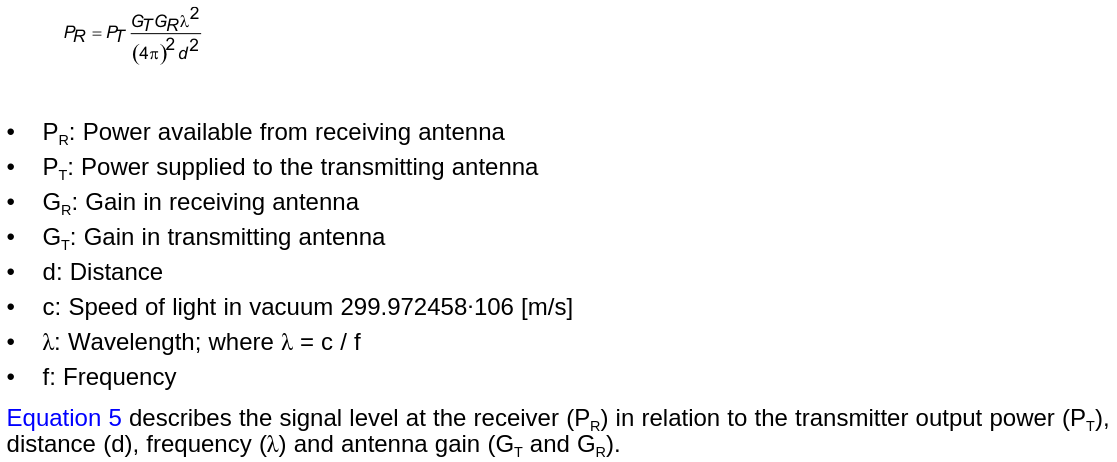
\includegraphics[width=0.8\textwidth]{assets/Friis.png}
	\caption{}
	\label{fig:friis}
\end{figure}


\subsection{Selection}
There are not many transcievers chips avaliable,
more modules. Chips would require design and measurement of the antenna matching circuit,
but also could possibly compensate an antenna missmatch.
\begin{itemize}
	\item CC1121/5 digital and well documented. Requires PA like SMA70-2
	\item SA818-U looks like trash because it is. Analog FM
	\item SX1261/2 150 MHz - 960 MHz
	\item Si446x (119–1050 MHz), looks perfect, reddit says is a bit buggy.
	\item AX5043 Good things on the internet. N.A and Dead but apperently good
\end{itemize}

\subsection{CC1121/5}
Pin compatible Chips, CC1125 has a more narrow band than CC1121 so is to be preferred.
Can be paired with a power amplifier like Gali 74+ to get +38 dBm :) \href{https://www.youtube.com/watch?v=9ZoO_AABzqU&t=313s}{youtube link}

\begin{figure}[H]
    \centering
    \begin{minipage}{0.48\textwidth}
        \centering
        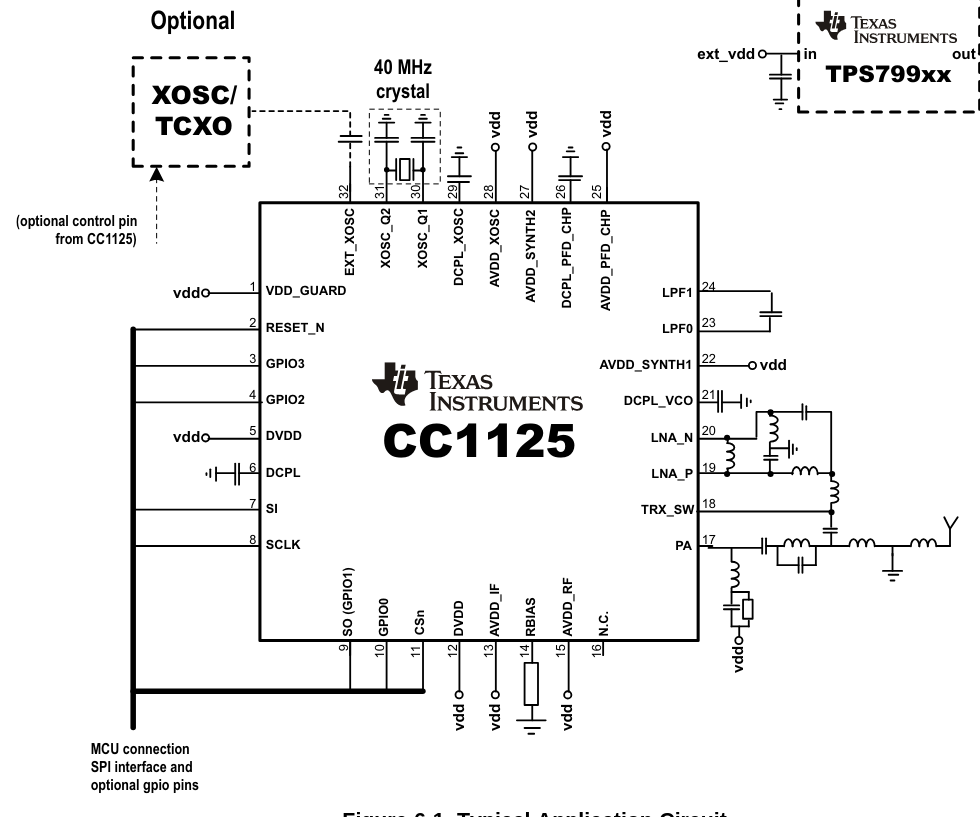
\includegraphics[width=\textwidth]{assets/CC1125.png}
        \caption{}
        \label{fig:cc1125}
    \end{minipage}
    \hfill
    \begin{minipage}{0.48\textwidth}
        \centering
        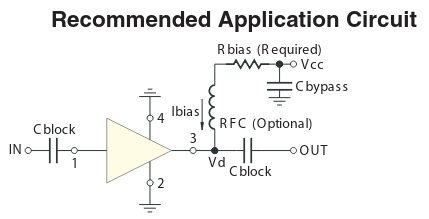
\includegraphics[width=\textwidth]{assets/Gali74.png}
        \caption{Gali74 application circuit}
        \label{fig:gali74}
    \end{minipage}
\end{figure}

\subsection{SA818-U}
RDA1846 (8 dBm) chip + PA + microcontroller. \href{http://ptptelecom.com/openlmrorg/Tiny_Transcievers.html}{Disassembly}
\begin{figure}[H]
	\centering
	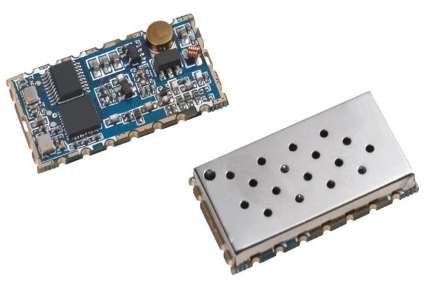
\includegraphics[width=0.4\linewidth]{./pics/SA818.png}
	% \caption{Birds}
\end{figure}

\subsection{Si446x}
\begin{figure}[H]
	\centering
	
\includegraphics[width=0.4\linewidth]{./pics/si.png}
	% \caption{Birds}
\end{figure}

\section{Antenna}

\subsection{Mechanical considerations}
Length estimate:\\
regarding the conductor as an open-ended single wire transmission line (resonant stub):
\[
	l_{\text{monopole}} = \frac{\lambda}{4} = \frac{c}{4f} = \frac{300}{4f\,[\text{MHz}]} = \frac{75}{f\,[\text{MHz}]}\,\text{m}
\]
Frequency of around 150 MHz -> length of around 0.5 m.

Requirements:
\begin{itemize}
	\item Non ferro magnetic
	\item around .5 m long
\end{itemize}

Spring based system:
\begin{figure}[H]
	\centering
	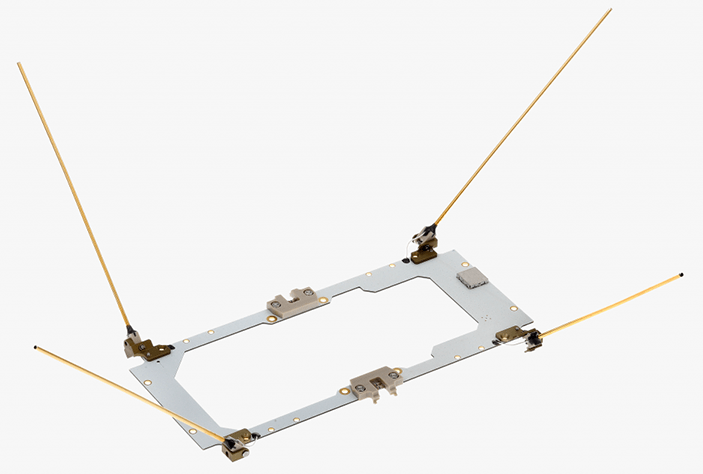
\includegraphics[width=0.4\linewidth]{spring.png}
	% \caption{Birds}
\end{figure}

Roll based system:
\begin{figure}[H]
	\centering
	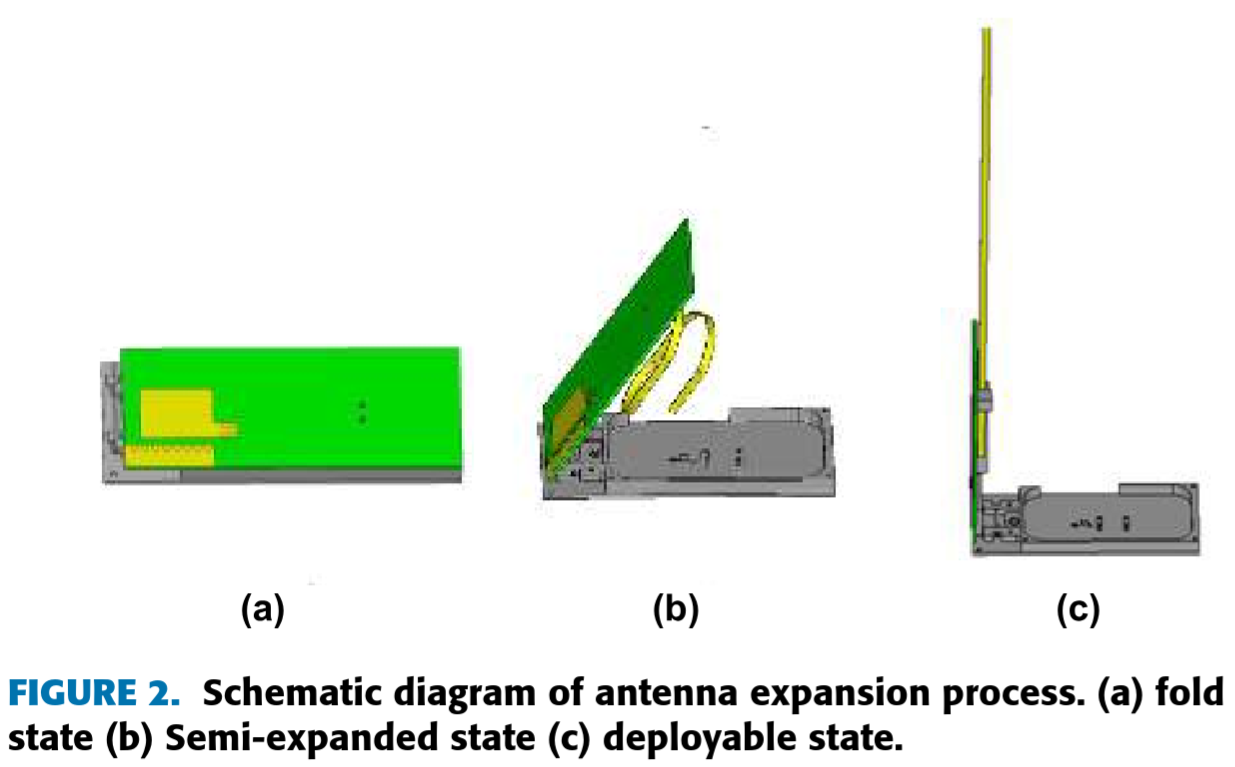
\includegraphics[width=0.4\linewidth]{fold.png}
	\caption{\href{https://www.researchgate.net/publication/342999505_Compact_UHFVHF_Monopole_Antennas_for_CubeSats_Applications}{paper}}
\end{figure}
\begin{figure}[H]
	\centering
	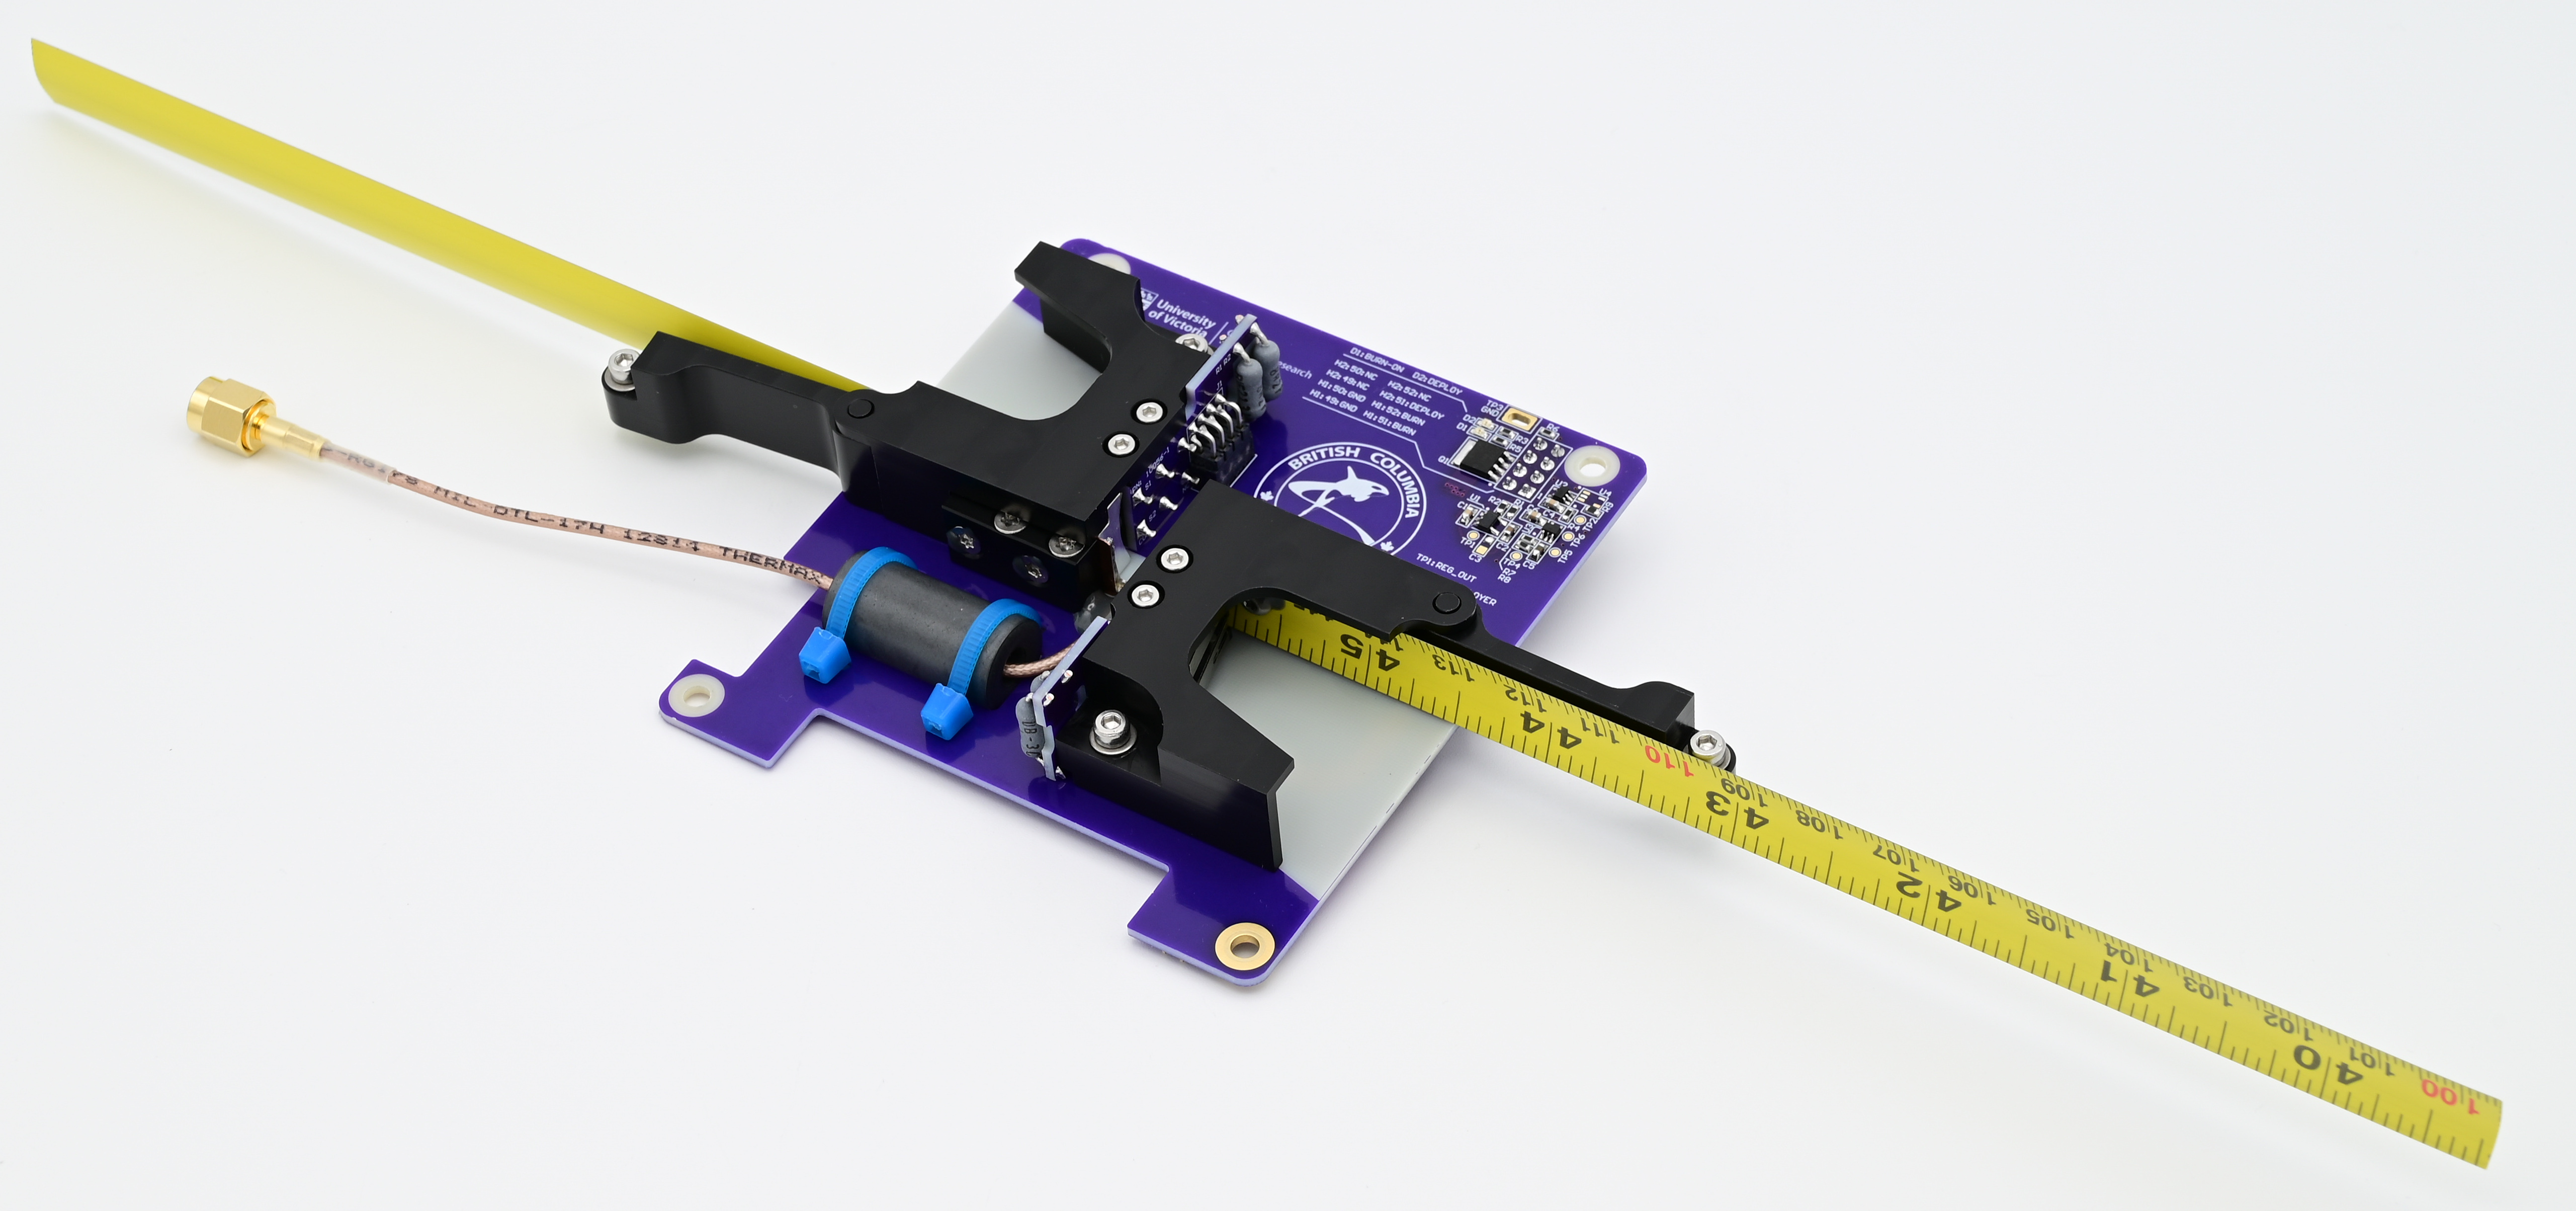
\includegraphics[width=0.4\linewidth]{spring.jpg}
	% \caption{Birds}
\end{figure}

\subsection{Material Choice}
\begin{itemize}
	\item strip steel. Used in tape measures. ferromagnetic but serves as comparison.
	\item 13RM19. strip steel but special non ferromagnetic. hard to obtain
	\item 1.4310. brother of 13RM19
	\item Beryllium copper (C17200). no way that this springs. on amazon
\end{itemize}

\begin{tabular}{lcccc}
	\toprule
	\textbf{material} & magnetization & Dehngrenze $R_{p0{,}2\%}$ & elastisity  & specific R \\
	                  &               & $N/mm ^ 2$                & $kN/mm ^ 2$              \\
	\midrule
	1.4310            & low           & 210                       & 200                      \\
	                  &               &                           &                          \\
	                  &               &                           &                          \\
	\bottomrule
\end{tabular}

\subsection{Simulation}


\subsection{Testing}

\subsection{Relevant papers:}
\begin{itemize}
	\item \href{}{Compact UHF/VHF Monopole Antennas for CubeSats Applications}
	\item \href{}{}
\end{itemize}

% \end{multicols*}
\end{document}

